%------------------------------------------------------------------------------
% Template file for the submission of papers to IUCr journals in LaTeX2e
% using the iucr document class
% Copyright 1999-2013 International Union of Crystallography
% Version 1.6 (28 March 2013)
%------------------------------------------------------------------------------

\documentclass[preprint]{iucr}              % DO NOT DELETE THIS LINE
%\documentclass[]{iucr}              % DO NOT DELETE THIS LINE
\usepackage{amssymb}
\usepackage[fleqn]{amsmath}
\usepackage{graphicx}
\usepackage{calligra}
\DeclareMathAlphabet{\mathcalligra}{T1}{calligra}{m}{n}
\def\mathbi#1{\textbf{\em #1}}
\numberwithin{equation}{section}
\DeclareMathSymbol{\Gamma}{\mathalpha}{letters}{"00}
\DeclareMathSymbol{\Lambda}{\mathalpha}{letters}{"03}
\DeclareMathSymbol{\Omega}{\mathalpha}{letters}{"0A}
\DeclareMathAlphabet{\mathitbf}{OML}{cmm}{b}{it}
\hyphenation{Niggli}
\def\mathbi#1{\textbf{\em #1}}
\numberwithin{equation}{section}
\DeclareMathSymbol{\Gamma}{\mathalpha}{letters}{"00}
\DeclareMathSymbol{\Lambda}{\mathalpha}{letters}{"03}
\DeclareMathSymbol{\Omega}{\mathalpha}{letters}{"0A}
\DeclareMathAlphabet{\mathitbf}{OML}{cmm}{b}{it}
\usepackage{color}
%\usepackage{ulem}
\newcommand{\NKS}[1]{{\color{red}~\textsf{#1}}}
\usepackage{url}
\usepackage{booktabs}
%\usepackage{multirow}
%\usepackage{xr-hyper}
%\usepackage[draft]{hyperref}
%\usepackage{bibentry}
%-------------------------------------------------------------------------
% Information about journal to which submitted
%-------------------------------------------------------------------------
\journalcode{J}              % Indicate the journal to which submitted
%   A - Acta Crystallographica Section A
%   B - Acta Crystallographica Section B
%   C - Acta Crystallographica Section C
%   D - Acta Crystallographica Section D
%   E - Acta Crystallographica Section E
%   F - Acta Crystallographica Section F
%   J - Journal of Applied Crystallography
%   M - IUCrJ
%   S - Journal of Synchrotron Radiation
\makeatletter
\font\dummyft@=dummy \relax
\makeatother


\begin{document}                  % DO NOT DELETE THIS LINE
	
	%-------------------------------------------------------------------------
	% The introductory (header) part of the paper
	%-------------------------------------------------------------------------
	
	% The title of the paper. Use \shorttitle to indicate an abbreviated title
	% for use in running heads (you will need to uncomment it).
	
	% Authors' names and addresses. Use \cauthor for the main (contact) author.
	% Use \author for all other authors. Use \aff for authors' affiliations.
	% Use lower-case letters in square brackets to link authors to their
	% affiliations; if there is only one affiliation address, remove the [a].
	
	% Use \vita if required to give biographical details (for authors of
	% invited review papers only). Uncomment it.
	
	% lca IUCr id IUCr6401
	% HJB IUCr id IUCr6484
	% NKS IUCr ID: IUCr7572
	% lca ORCID  0000-0002-4451-1641
	% HJB ORCID 0000-0002-0517-8532
	% NKS ORCID 0000-0003-2786-6552
	%\vita{Author's biography}
	
	% Keywords (required for Journal of Synchrotron Radiation only)
	% Use the \keyword macro for each word or phrase, e.g. 
	% \keyword{X-ray diffraction}\keyword{muscle}
	
	
	% PDB and NDB reference codes for structures referenced in the article and
	% deposited with the Protein Data Bank and Nucleic Acids Database (Acta
	% Crystallographica Section D). Repeat for each separate structure e.g
	% \PDBref[dethiobiotin synthetase]{1byi} \NDBref[d(G$_4$CGC$_4$)]{ad0002}
	
	%\PDBref[optional name]{refcode}
	%\NDBref[optional name]{refcode}
	
	%-------------------------------------------------------------------------
	% The introductory (header) part of the paper
	%-------------------------------------------------------------------------
	
	% The title of the paper. Use \shorttitle to indicate an abbreviated title
	% for use in running heads (you will need to uncomment it).
	{\LARGE \emph{\today}} \\
	\title{Approximating Lattice Similarity}
	%\title{Note on the transformation of three-space basis vectors to  corresponding matrix for Delaunay scalars}
	\shorttitle{Lattice Matching}
	
	% Authors' names and addresses. Use \cauthor for the main (contact) author.
	% Use \author for all other authors. Use \aff for authors' affiliations.
	% Use lower-case letters in square brackets to link authors to their
	% affiliations; if there is only one affiliation address, remove the [a].
	
	
	\cauthor[a]{Lawrence C.}{Andrews}{lawrence.andrews@ronininstitute.org}{}
	\author[b]{Herbert J.}{Bernstein}
	\author[c]{Nicholas K.}{Sauter}
	
	\aff[a]{Ronin Institute, 9515 NE 137th St., Kirkland, WA, 98034-1820 \country{USA}}
	\aff[b]{Ronin Institute, c/o NSLS-II, Brookhaven National Laboratory, Upton, NY, 11973-5000 \country{USA}}
	\aff[c]{Lawrence Berkeley National Laboratory, 1 Cyclotron Rd., Berkeley, CA, 94720 \country{USA}}
	
	% Use \shortauthor to indicate an abbreviated author list for use in
	% running heads (you will need to uncomment it).
	
	\shortauthor{Andrews, Bernstein, and Sauter}
	
	% Use \vita if required to give biographical details (for authors of
	% invited review papers only). Uncomment it.
	
	% lca IUCr id IUCr6401
	%\vita{Author's biography}
	
	% Keywords (required for Journal of Synchrotron Radiation only)
	% Use the \keyword macro for each word or phrase, e.g. 
	% \keyword{X-ray diffraction}\keyword{muscle}
	
	\keyword{Lattice Matching}
	\keyword{Delaunay}
	\keyword{Delone}
	\keyword{Niggli}
	\keyword{Selling}
	
	% PDB and NDB reference codes for structures referenced in the article and
	% deposited with the Protein Data Bank and Nucleic Acids Database (Acta
	% Crystallographica Section D). Repeat for each separate structure e.g
	% \PDBref[dethiobiotin synthetase]{1byi} \NDBref[d(G$_4$CGC$_4$)]{ad0002}
	
	%\PDBref[optional name]{refcode}
	%\NDBref[optional name]{refcode}
	
	\maketitle                        % DO NOT DELETE THIS LINE
	
	\begin{synopsis}
		A method is proposed for transforming unit cells for a group of crystals so that they all appear
		as similar as possible to a selected cell.
	\end{synopsis}
	
	\newcommand{\OPES}[0]{$E^3toS^6$}
	\newcommand{\OPESS}[0]{$$E^3toS^6$$}
	\newcommand{\SVI}[0]{$\bf{S^{6}}$}
	\newcommand{\GVI}[0]{$\bf{G^{6}}$}
	\newcommand{\CIII}[0]{$\bf{C^{3}}$}
	\newcommand{\EIII}[0]{$\bf{E^{3}}$}
	\newcommand{\RIII}[0]{$\bf{R^{3}}$}
	\newcommand{\DVII}[0]{$\bf{D^{7}}$}
	\newcommand{\VVII}[0]{$\bf{V^{7}}$}
	\newcommand{\MSVI}[0]{$M_{S^{6}}$}
	\newcommand{\MEIII}[0]{$M_{E^{3}}$}
	\newcommand{\EXIII}[0]{$\bf{E^{3 \times 3}}$}
	\newcommand{\scalarsub}[2]{$#1_#2$}
	\newcommand{\vdotv}[2]{${{\bf #1 \cdot #2}}$}
	
	\begin{abstract}
		
		A method is proposed for choosing unit cells for a group of crystals so that they all appear
		as nearly similar as possible to a selected cell. Related unit cells with varying cell parameters 
		or indexed with different lattice centering can be accommodated.
		
	
		
	\end{abstract}
	
	%-------------------------------------------------------------------------
	% The main body of the paper
	%-------------------------------------------------------------------------
	% Now enter the text of the document in multiple \section's, \subsection's
	% and \subsubsection's as required.
	
	
	
	
	% Appendices appear after the main body of the text. They are prefixed by
	% a single \appendix declaration, and are then structured just like the
	% body text.
	
	
	\section{Introduction}
	
	A common problem in crystallography is to provide a list of the unit cells of several (or many) 
	crystals so that they can be visually compared, making it easier to identify meaningful clusters
	of crystals of related morphology. Collections of experimental unit cell parameters have 
	been created based on similarity of morphology (for example, see \citeasnoun{Donnay1963}), and,
	in recent years, the clustering of unit cells from the
	myriad of images in serial crystallography has become increasingly important \cite{keable2021room}. We have created a method
	to group unit cells to serve these needs and have addressed this problem in the space \SVI{} \cite{Andrews2019b}.
	
	\section{Background and notation}
	
	\subsection{The space \SVI{}}
	\citeasnoun{Andrews2019b} introduced the space \SVI{} as an alternative
	representation of crystallographic lattices. The space is defined in terms of the
	``Selling scalars'' used in Selling reduction \cite{Selling1874} and by \citeasnoun{Delaunay1932}%
		\footnote{In his later publications, Boris Delaunay used the Russian version of his surname, Delone.}
	for the classification of lattices. A point $\bf{s}$ in \SVI{} is defined by 
	
	$\bf{s}$  = [\vdotv{b}{c}, \vdotv{a}{c}, \vdotv{a}{b}, \vdotv{a}{d}, \vdotv{b}{d}, \vdotv{c}{d}]
	where
	${\mathbf d} = -{\mathbf a} - {\mathbf b} - {\mathbf c}$.
	As a mnemonic to remember the order: the terms involve, in order, $ \alpha, \beta,
	\gamma, \mathbf{a}, \mathbf{b}, \mathbf{c}$.
	
%	\subsection{The space \GVI{}}
%	\citeasnoun{Andrews2014} introduced the space \GVI{} based on the metric tensor
%	and operated on by Niggli reductions \cite{Niggli1928}. A point in \GVI{}
%	is defined by \\
%	$\bf{g}$ =   [$\mathit{a^2}$, $\mathit{b^2}$, $\mathit{c^2}$, 2\vdotv{b}{c}, 2\vdotv{a}{c}, 2\vdotv{a}{b}]
	
	\subsection{Similarity}
	
In Euclidean geometry, two objects are described as ``similar'' if they are identical except for a scale factor, see Euclid, in \cite{heath1956thirteen}.
	In crystallography, we can say that all face-centered cubic unit cells are similar (assuming
	that they are in the same presentation). On the other hand, not all primitive orthorhombic 
	unit cells are similar.  In a metric space, we
	refer to two objects as ``approximately similar'' if the distance between them after scaling
	to the same size is, in some sense, small, {\it e.g}. commensurate with the experimental errors
	in determination of the unit cells.  The algorithm below attempts to find the representation of one 
	cell that is nearest-to-similar to some other cell. For a given reference cell, the probe cell
	will be transformed to other choices of unit cell that would generate the probe's lattice, and the
	closest match to the reference will be chosen for the result. Finally, the lattice centering
	of the reference cell will be restored (if necessary).
	
	\section{Algorithm}
	
	We start with a collection of experimental unit cells. From among them, we select or create the
	``reference'' cell; that is the one to which all the rest will be matched as closely as possible.
	
	We transform the reference cell by many operations in the course of exploring alternative
	lattice representations. For each newly
	generated lattice representation, we accumulate the transformations needed to convert  back to the 
	original reference cell.  All of these operations are
	performed in \SVI{}. (The alternative space, \GVI{}, is less convenient
	because the $ \mathbf{G^6}$ fundamental unit is non-convex.) To avoid duplication, for each step 
	we only accumulate transformations
	that have not already been found. 
	
	To begin, each input cell is transformed to the \SVI{} representation, and then 
	Selling-reduced (see \citeasnoun{Delaunay1932} and \citeasnoun{Andrews2019a}). As
	there is a need to be able to reverse the reduction, the reduction transformation 
	is saved for use in later stages.
	
	The following transformations of the reference will be done in three stages.
	
	First, the 24 \SVI{} reflections are
	applied \cite{Andrews2019b} and the results stored. The store of \SVI{} vectors and their generating matrices holds 24 entries each at that point.
	
	Because the 24 operations defining reflection are unitary and
	in \SVI{} they are simply perturbations of the six values,
	they retain the values and signs of he six values, 
	simply rearranging the six scalars.
	
	
	Next the boundary (reduction) transformations \cite{Andrews2019b} are applied to
	the results of the previous step. Then, the 24 reflections are applied again. In
	each step, only newly found results are stored. These latter two steps are repeated 
	at least once in order to gain better coverage of possibly useful transformations. 
	The counts of entries for each iteration are 24, 1566, 45876, and finally 1016726.
	Three iterations, {\it i.e.} 45876 entries, have been sufficient in test cases to date.
	
	Although the six scalars are all negative for Selling
	reduced unit cells, the boundary transformations are
	not unitary, and so not retain the six negative values.
	
	
	Next, all the accumulated, transformed representations of the reference cell must be rescaled and the saved
	transformations inverted.
	The \SVI{} vectors are all scaled to the same length (see Section~\ref{section:modified}), and the transformation matrix
	attached to each vector is inverted, thereby yielding the operation to return a lattice to the vicinity of the
	original reference cell. For more efficient searching in the final step, it is helpful to use
	a nearest neighbor search function such as NearTree \cite{andrews2016}.
	
	\section{Why must the \SVI{} vectors be scaled?} 	\label{section:modified}
	
	All similar lattices lie on lines that go through the origin of \SVI{}. Fig. \ref{similarity} shows
	the distinction between the cases where the transformed points are scaled to all be at the same
	distance from the origin as the reference point ( Fig. \ref{similarity}\textbf{a}) and the case where they are not ( Fig. \ref{similarity}\textbf{b}).
	Fig. \ref{zone} illustrates the way in which scaling all the reference points to the same
	6-spherical surface defines the zones of approximate similarity.
	Any non-zero scale factor will produce the same correct result. In \SVI{}
	the reflections maintain the distance from the origin, but the boundary transformations may not.
	Repeating: the only way to guarantee that the
	separation line for two regions goes through the origin is to have all the points at
	the same radius.
	
	\begin{figure}
		\label{similarity}
		
\includegraphics[height=3.8cm]{similarity}
		\caption{Frame \textbf{a} shows the case where the transformed point \textbf{T} has been scaled to be at the same distance 
			from the origin as the reference point \textbf{R}.  In Frame \textbf{b}, point \textbf{T} has not been scaled, and some areas
			are incorrectly assigned to point R.  In each frame, the straight line between points \textbf{R} and \textbf{T} separates the 
			regions closer to each of the points.}
	\end{figure}
	
	\begin{figure}
		\label{zone}
		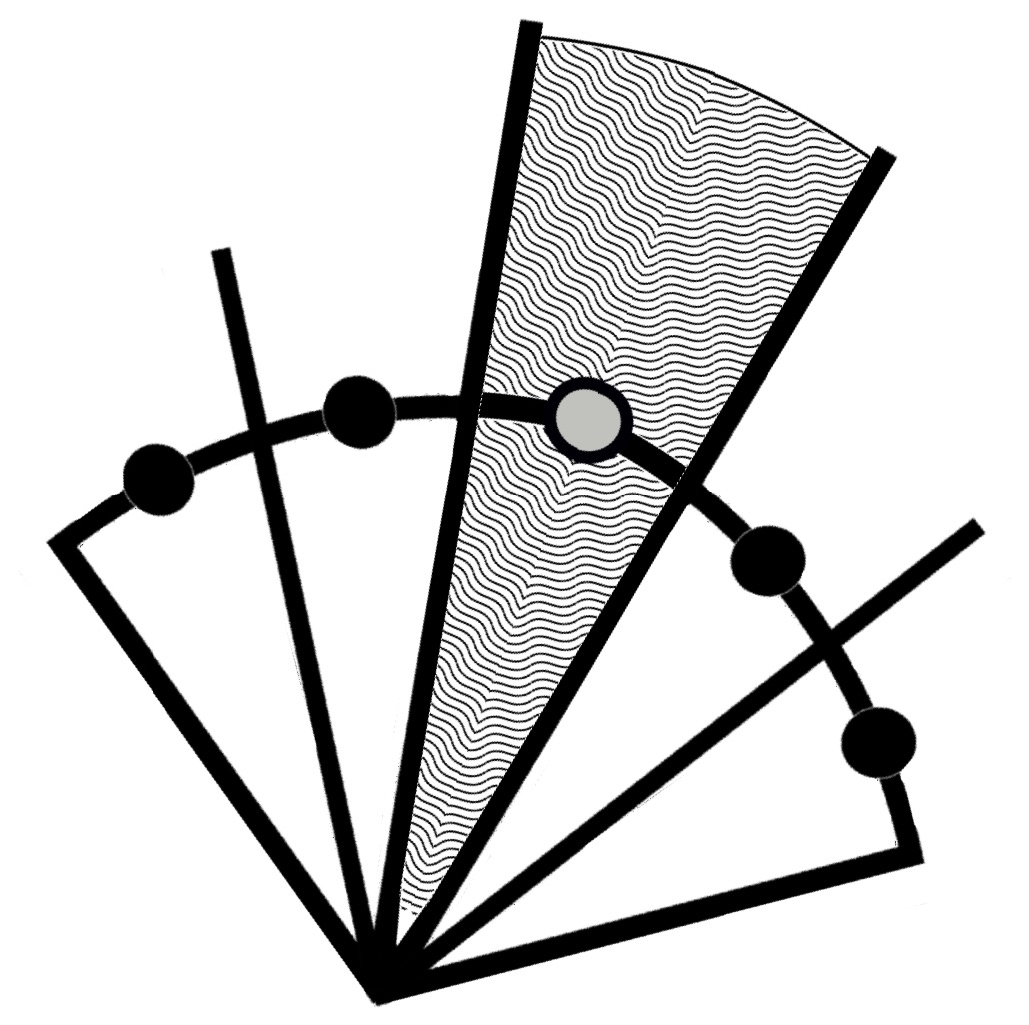
\includegraphics[height=5cm]{zone2a}
		\caption{A two-dimensional example of the determining similarity. Each transformed copy of the reference cell
			is normalized to a constant length in the chosen space (here, \SVI{}). Each transformed and normalized cell then 
			defines a zone in which every point in that zone is closer to the transformed and normalized cell defining that zone than it is
			to the transformed and normalized cell defining any other zone.  In this example, each point within the textured zone (which extends
			to infinity) is closer to the
			gray-centered point than it is to any of the black points.}
	\end{figure}

\section{Angular measure of fit}

Because the measure of similarity is independent of scale, projecting
points onto a spherical surface does not modify the similarity. The
angle between a probe point and the reference point is a meaningful measure of how
similar the two points are.
	
	\section{Generating the approximation}
	
	The following operations are performed for each of the probe lattices in 
	the original list.  For a given probe lattice, the closest approximation among all of the 
	transformed reference points is found. If there are multiple representations of the 
	reference point that are equally close, then all should be examined. For the case of multiples, a
	method must be used to find the preferred one. For our purposes, we have found
	it convenient to choose the one for which the unreduced \GVI{} distances to the transformed
	reference is the smallest. Other choices might be useful for other purposes.
	
	Once the preferred result has been found, the corresponding inverted transformation is used
	to place the vector in the region of the original reduced reference cell. Finally, the inverse of the reduction
	operation that was performed on the reference cell is used to create the best match
	to the original reference. If it is desirable to restore lattice centering, then that operation must also  be
	performed; the search returns a primitive representation
	of the unit cell.
	
	\section{Examples}
	\subsection{A rhombohedral example}
	\citeasnoun{LeTrong2007} cite several structures for phospholipase A2 (krait neurotoxin) that were reported as 
	different structures but were actually all the same structure \cite{bernstein2020}. Expanding their search using the program SAUC 
	\cite{mcgill2014},
	we find a total of six structures, four of which are identical in 
	two pairs. Table \ref{table:LT1} lists the unit cells as reported in the Protein
	Data Bank \cite{Bernstein1977} \cite{Berman2000}. In Tables \ref{table:LT2}, \ref{table:LT3}, and \ref{table:LT4}, the first
	entry in each table is used as the reference, and the following five entries are matched as 
	closely as possible to the presentation of the reference cell. In Table \ref{table:LT2}, a
	rhombohedral presentation 1DPY was chosen as the reference. In Table \ref{table:LT3},
	C-centered cell 1G2X was chosen as the reference. In Table \ref{table:LT4}, the hexagonal cell 1U4J
	was chosen as the reference. In each case, the probe cells
	were return in the same presentation, including lattice 
	centering as the reference cell. So the resulting centerings
	were hR, mC, and hP, respectively, for each matched cell,
	regardless of the input centering, which had been determined
	by crystallographic analysis.
	~~\\
	
	\begin{table}
		\begin{center}
			\caption{Unit cells of phospholipase A2 from the Protein Data Bank.}		
			\vspace{3mm}
			\begin{tabular}{lccccccccccc}
				\toprule
				PDB &   & a &b &c&$\alpha$&$\beta$&$\gamma$ \\
				\midrule
				1DPY &R& 57.98& 57.98 &57.98 &92.02  &92.02 &92.02 \\ 
				1FE5 &R& 57.98& 57.98 &57.98 &92.02  &92.02 &92.02 \\ 
				1G0Z &H& 80.36& 80.36 &99.44 &90     &90    &120   \\ 
				1G2X &C& 80.95& 80.57 &57.1  &90     &90.35 &90    \\ 
				1U4J &H& 80.36& 80.36 &99.44 &90     &90    &120   \\ 
				2OSN &R& 57.10 & 57.10  &57.10  &89.75  &89.75 &89.75  \\ 
				\bottomrule
			\end{tabular}
			\label{table:LT1}
		\end{center}
	\end{table}	
	
	
	\begin{table}
		\begin{center}
			\caption{The data of Table \ref{table:LT1} matching a rhombohedral reference. The 
				reference cell is marked in boldface.}
			\vspace{3mm}
			\begin{tabular}{lccccccccccc}
				\toprule
				PDB &   a & b & c & $\alpha$ & $\beta$ & $\gamma$ & fit(degrees) \\ \midrule
\textbf{1DPY} & \textbf{57.98}  & \textbf{57.98}  & \textbf{57.98}  &
\textbf{92.02}  & \textbf{92.02}  & \textbf{92.02} & 0 \\ 
1FE5 &57.980& 57.980 & 57.980 & 92.020 & 92.020 & 92.020 & 0    \\
1G0Z &57.020& 57.020 & 57.020 & 90.395 & 90.395 & 89.605 & 2.11 \\
1G2X &57.106& 57.106 & 57.100 & 89.752 & 90.248 & 90.270 & 2.11 \\
1U4J &57.020& 57.020 & 57.020 & 90.395 & 90.395 & 89.605 & 2.11 \\
2OSN &57.100& 57.100 & 57.100 & 90.250 & 90.250 & 89.750 & 2.11 \\

				\bottomrule
			\end{tabular}		
			\label{table:LT2}
		\end{center}
	\end{table}	
	
	
	\begin{table}
		\begin{center}
			\caption{The data of Table \ref{table:LT1} matching a monoclinic reference. The 
				reference cell is marked in boldface.}
			\vspace{3mm}
			\begin{tabular}{lccccccccccc}
				\toprule[1pt]
								PDB &   a & b & c & $\alpha$ & $\beta$ & $\gamma$ & fit(degrees) \\ \midrule
\textbf{1G2X} & \textbf{80.95}  & \textbf{80.57}0  & \textbf{57.10}  & \textbf{90}  & \textbf{90.35}  & \textbf{90} & \textbf{0}   \\
1DPY & 83.42999  & 80.53835  & 57.98115  & 87.0908  & 89.9992  & 90.00114 & 3.14          \\
1FE5 & 83.42999 &  80.53835  & 57.98115  & 87.0908  & 89.9992  & 90.00114 & 3.14          \\
1G0Z & 80.91861  & 80.35937  & 57.02143  & 89.9996  & 90.5644  & 90.00144 & 0.09        \\
1U4J & 80.91861  & 80.35937  & 57.02143  & 89.9996  & 90.5603  & 90.00144 & 0.09       \\
2OSN & 80.92799  & 80.57842  & 57.10254  & 90.0002  & 90.3502  & 89.99745 & 0.01      \\

				\bottomrule[1pt]
			\end{tabular}
			\label{table:LT3}
		\end{center}
	\end{table}	
	
	
	\begin{table}
		\begin{center}
			\caption{The data of Table \ref{table:LT1} matching a hexagonal reference. The reference cell is marked in boldface.}
			\vspace{3mm}
			\begin{tabular}{lccccccccccc}
				\toprule
PDB &   a & b & c & $\alpha$ & $\beta$ & $\gamma$ & fit(degrees) \\ \midrule         
\textbf{1U4J} & \textbf{80.36} & \textbf{80.36} & \textbf{99.44} & \textbf{90} & \textbf{90} & \textbf{120} & \textbf{0} \\
1DPY & 83.4287 & 80.5380 & 101.5974 & 91.6597 & 90 & 121.195 & 4.30   \\
1FE5 & 83.4287 & 80.5380 & 101.5974 & 91.6597 & 90 & 121.195 & 4.30   \\
1G0Z & 80.3600 & 80.3600 & 99.4400  & 90 & 90 & 120 & 0          \\
1G2X & 80.5809 & 80.5809 & 99.3468  & 90.0138 & 89.986 & 120.009 & 0.09  \\
2OSN & 80.5752 & 80.5752 & 99.3307  & 90 & 90 & 120 & 0.08  \\

				\bottomrule
			\end{tabular}		
			\label{table:LT4}
		\end{center}
	\end{table}	
	
	
	\subsection{Adenosine receptor A2A}
	Unit cells were determined automatically from frames from serial crystallography data collection for adenosine receptor A2A, PDB ID: 5NLX, \cite{weinert2017}.
	
	Three example unit cells were chosen from several hundred indexed data frames.
	Two are C-centered and one is primitive. 
	Table \ref{table:signal0} is the reported data, and tables
	\ref{table:signal1}, \ref{table:signal2}, and \ref{table:signal3}
	are the approximate similarity matches.
	\begin{table}
		\begin{center}
			\caption{Adenosine receptor A2A: 5NLX, unit cells as reported.  }
~~\\
			
			\begin{tabular}{clccccccccccc}
				\toprule
				serial\\
				\midrule
				1&C&39.741&183.767&140.649&90&90&90.\\
				2&P&40.160&142.899&92.417&90&102.480&90.\\
				3&C&180.613&40.156&142.737&90&90.017&90.\\
				\bottomrule 
			\end{tabular}
			\label{table:signal0}
		\end{center}
	\end{table}

	\begin{table}
		\begin{center}
			\caption{Adenosine receptor A2A:  Approximating a C-centered cell.
				The reference cell is marked in boldface.
				 Centering in parentheses indicates the lattice centering before matching.}
			\vspace{3mm}
			\begin{tabular}{clccccccccccc}
				\toprule
serial&center &a & b & c & $\alpha$ & $\beta$ & $\gamma$ & fit(degrees) \\ \midrule         
1&\textbf{C}    & \textbf{39.741} & \textbf{183.767} & \textbf{140.649}  & \textbf{90}  &\textbf{90}  &\textbf{90} &  \textbf{0}\\
2&(P)  & 40.160 & 180.467 & 142.899  & 90  & 90  & 89.931 & 1.37981\\
3&C    & 40.156 & 180.613 & 142.737  & 89.983  & 90  & 90 &  1.30423\\
				\bottomrule
			\end{tabular}
		\end{center}
	\label{table:signal1}
	\end{table}
	
	
	\begin{table}
		\begin{center}
			\caption{Adenosine receptor: A2A. Approximating a primitive cell.   The reference cell	is marked in boldface.  Centering in parentheses indicates the lattice centering before matching.}
			~~\\c

			
			\begin{tabular}{lccccccccccc}
				\toprule
serial&center& a & b & c & $\alpha$ & $\beta$ & $\gamma$ & fit(degrees) 	\\			
\toprule
				2&\textbf{P} & \textbf{40.160} & \textbf{142.899} & \textbf{92.417} & \textbf{90} & \textbf{102.480} & \textbf{90}&\textbf{0}	\\  
1&(C)   & 39.741 & 140.649  & 94.008  & 90 &  102.21  & 90 &  1.37981 \\
3&(C)   & 40.156 & 142.73  & 92.512  & 89.983 & 102.535 & 90 &  0.08374 \\				\bottomrule
			\end{tabular}
		\end{center}
	\label{table:signal2}
	\end{table}

%	\begin{table}
%		\vspace{3mm}
%		\begin{center}
%			\begin{tabular}{lccccccccccc}
%				\toprule
%				P &	\textbf{40.160}& \textbf{142.899} & \textbf{92.417} &
%				\textbf{90.} &\textbf{102.480} & \textbf{90.} \\
%				C  & 39.741 & 140.649 & 94.008 & 90. & 102.203 & 90.   \\
%				C  & 40.156 & 142.737 & 92.512 & 89.983 & 102.535 & 90.   \\ 
%				\bottomrule
%			\end{tabular}			
%			\label{table:signal2}
%		\end{center}
%	\end{table}	
	
%	\begin{table}
%		\begin{center}
%			\caption{Adenosine receptor: A2A. Approximating a C-centered alternate presentation.   
%				The reference cell is marked in boldface.}
%			\vspace{3mm}
%			\begin{tabular}{lccccccccccc}
%				\toprule
%				C & 180.613 & 40.156 & 142.737 & 90. & 90.017 & 90. \\ 
%				C &  39.741& 183.767& 140.649 & 90. & 90. & 90 \\  
%				P &  40.160 &142.899 & 92.417 & 90. &102.480 & 90. \\ 
%				\bottomrule
%			\end{tabular}			
%		\end{center}
%	\end{table}
	
	\begin{table}
		\begin{center}
			\caption{Adenosine receptor: A2A. Approximating a C-centered cell.   The reference cell	is marked in boldface.  Centering in parentheses indicates the lattice centering before matching.}
			~~\\
			
			\begin{tabular}{clccccccccccc}
				\toprule
serial&center& a & b & c & $\alpha$ & $\beta$ & $\gamma$ & fit(degrees) \\
\midrule
				3&	\textbf{C} &  \textbf{180.613} &  \textbf{40.156} & \textbf{142.737} &  \textbf{90} &   \textbf{90.017} &  \textbf{90} &\textbf{0}  \\
			1&	C &  183.767 &  39.741 & 140.649 &  90 &  90 &  90 &1.31 \\
			2&	(P) &  180.467 &  40.160 & 142.899 &  90 &  90 &  89.930 &0.07\\
				\bottomrule
			\end{tabular}
			\label{table:signal3}
		\end{center}
	\end{table}	
	
	
	
	
	\subsection{Points along a line in \SVI}
	Tables \ref{table:AD1} and \ref{table:AD2} present two views of artificial data. 
	A line of points in \SVI{} was created from the C-centered [80.95, 80.95, 57.10, 90, 90.35, 90] 
	to the A-centered [57.10, 80.95, 80.95, 90, 90, 90.35] representation of the same cell of phospholipase A2. The 
	series of intervening points  interpolated in S6 and shown in Table \ref{table:AD1} (each as the reduced unit cell except for the endpoints), 
	and the lattice-matched results are shown
	in Table \ref{table:AD2}.
	
	In Table \ref{table:AD2},
	the first line is the reference cell. In both cases that is the C-centered cell above.
	The final cell is the same cell but in the A-centered presentation. The points between
	are equally spaced points in \SVI{} between those two centered points. Table \ref{table:AD1}
	presents the list of points as generated, and Table \ref{table:AD2} lists the same cells in the lattice-matching
	presentation. Because the initial cell was C-centered, the following cells are also
	in that presentation, although the intermediate cells are not C-centered.
	

			
	\begin{table}
		\begin{center}
			\caption{A line of unit cells generated by interpolating 
				between the first and last points in \SVI.}
			~~\\
					
			\begin{tabular}{lccccccccc}
				\toprule
				&a&b&c&$\alpha$&$\beta$&$\gamma$ \\ \midrule
				C & 80.95    &  80.95  & 57.1    &  90      &  90.35   & 90    \\  
				P & 57.24 &57.24 &80.68 &129.50 &94.21   &90     \\  
				P & 57.24 &57.24 &80.68 &124.46 &98.26  & 90    \\  
				P & 57.24 &57.24 &80.68 &119.70 &102.36 &90     \\  
				P & 57.24 &57.24 &80.68 &115.16 &106.52 &90     \\  
				P & 57.24 &57.24 &80.68 &110.78 &110.78 &90     \\  
				P & 57.24 &57.24 &80.68 &106.53 &115.16 &90     \\  
				P & 57.24 &57.24 &80.68 &102.36 &119.70 &90     \\ 
				P & 57.24 &57.24 &80.68 &98.26  &124.46 &90     \\  
				P & 57.24 &57.2& 80.68 &94.209   &129.50 &90  \\ 
				A &  57.10 & 80.95 & 80.95 & 90 & 90 & 90.35		\\	 
				\bottomrule
			\end{tabular}			
			\label{table:AD1}
		\end{center}
	\end{table}	
	
	
	\begin{table}
		\begin{center}
			\caption{Table 13 lists the same cells in the same order after transformation to approximately match the reference cell.
				The reference cell is marked in boldface.}
			\vspace{3mm}
			\begin{tabular}{ccccccccc}
				\toprule
 a & b & c & $\alpha$ & $\beta$ & $\gamma$ & fit(degrees) \\ \midrule         
\textbf{80.950} & \textbf{80.950}  &  \textbf{57.100}  & \textbf{90}  & \textbf{90.350}    & \textbf{90} & \textbf{0}  \\   
80.680 & 88.685  &  57.240  & 86.171  & 94.210    & 95.086 & 5.687  \\
80.680 & 95.7216  & 57.240  & 83.0450  & 98.260    & 99.564 &  12.17  \\
80.680 & 102.287 &  57.240 &  80.280 &  102.360  & 103.547 &  19.35  \\
80.680 & 108.450 &  57.240 &  77.787 &  106.520  & 107.167 & 27.08  \\
80.677 & 114.284 &  57.240 &  75.499 &  110.775  & 110.520 & 35.10  \\
80.680 & 108.450 &  57.240 &  77.780 &  106.530  & 107.167 & 27.09  \\
80.680 & 102.287 &  57.240 &  80.280 &  102.360  & 103.547 &  19.35  \\
80.680 & 95.722  &  57.240  & 83.045  & 98.260    & 99.564 &  12.17  \\
80.680 & 88.685  &  57.200  & 86.172  & 94.209    & 95.086 & 5.70  \\
80.950 & 80.950  &  57.100  & 90  & 90.350    & 90 & 0  \\
				\bottomrule
			\end{tabular}			
			\label{table:AD2}
		\end{center}
	\end{table}	
	
	\subsection{Examples from the Protein Data Bank}
	
	The program SAUC \cite{mcgill2014} was used to query the
	Protein Data Bank (PDB). The search started from the
	C-centered unit cell of PDB entry 1RGX (resistin) requesting the nearest 50 cells;
	26 unique cells resulted. Because there was no limit on
	how far the points could be from the probe, some cells
	differ significantly from the search cell. The results are listed
	in Table \ref{table:PDB1} in their published representation. Table \ref{tablePDB2} lists the same cells
	in the same order as in Table \ref{table:PDB1}, but with 
	the same lattice centering as 1RGX, which is the first, 
	reference entry.
	
	\begin{table}
		\begin{center}
			\caption{Unit cells from the Protein Data Bank. Cells listed are nearest the C-centered cell of 1RGX and 
				keeping only one representative of each protein type. The search was performed 
				using the program SAUC.}		
			\vspace{3mm}
			\begin{tabular}{lcccccccclcccc} \toprule
				\rotatebox{0}{PDB}&& a&b&c&$\alpha$&$\beta$&$\gamma$ \\ \midrule
				1RGX  &  C &   49.021  &  52.475 &   96.609  &  90 &   96.53 &   90 \\
				1R8M &  P  & 33.429  & 95.775  & 33.665   & 90     & 101.67~  & 90   \\
				2FXO  & P  & 40.157  & 41.867  & 97.795   & 91.11  & 92.73   & 107.18 \\
				4RNE  & C  & 37.656  & 54.197  & 95.677   & 90     & 90      & 90    \\
				3MGD  & C  & 57.933  & 56.341  & 99.721   & 90     & 98.86   & 90   \\
				5YO3  & C  & 40.328  & 50.126  & 94.237   & 90     & 90      & 90   \\
				4GZN  & C  & 40.218  & 60.641  & 96.119   & 90     & 90      & 90   \\
				3VVW  & C  & 195.72  & 37.420  & 40.280   & 90     & 94.66   & 90   \\
				4BHV  & P  & 33.078  & 33.621  & 99.138   & 90     & 96.75   & 90   \\
				3IHU  & C  & 54.646  & 79.135  & 103.244~  & 90     & 102.08~  & 90   \\
				5WOU  & C  & 36.429  & 53.884  & 94.219   & 90     & 90      & 90   \\
				3NHM  & C  & 56.616  & 40.408  & 99.617   & 90     & 102.28~  & 90   \\
				5K2L  & P  & 29.130  & 29.130  & 94.257   & 90     & 90      & 90   \\
				3T47  & P  & 26.152  & 94.356  & 29.196   & 90     & 97.19   & 90   \\
				4RUV  & P  & 31.376  & 31.376  & 94.804   & 90     & 90      & 90   \\
				5ED9  & C  & 86.371  & 34.743  & 99.839   & 90     & 101.49~  & 90   \\
				1SIP  & C  & 32.180  & 62.520  & 95.760   & 90     & 90      & 90   \\
				2SAM  & C  & 62.700  & 32.200  & 96.100   & 90     & 90      & 90   \\
				1YTJ  & C  & 62.300  & 32.100  & 96.300   & 90     & 90      & 90   \\
				4HHX  & C  & 34.790  & 73.610  & 95.900   & 90     & 90      & 90   \\
				3W92  & P  & 31.760  & 33.552  & 94.998   & 90     & 90      & 90   \\
				167D  & P  & 33.200  & 33.200  & 96.040   & 90     & 90      & 120  \\
				4QEG  & P  & 31.237  & 31.237  & 93.848   & 90     & 90      & 90   \\
				2YGG  & C  & 200.700~ & 38.350  & 34.100   & 90     & 91.35   & 90   \\
				1OZ7  & P  & 37.966  & 95.258  & 42.611   & 90     & 112.58~  & 90   \\
				6NFS  & P  & 30.584  & 34.753  & 94.679   & 90     & 90      & 90   \\ \bottomrule
			\end{tabular}			
			\label{table:PDB1}
		\end{center}
	\end{table}
	
	
	\begin{table}
		\begin{center}
			\caption{Data in Table \ref{table:PDB1} best-matched to PDB entry 1RGX.  The 
				reference cell is marked in boldface.}
			\vspace{3mm}
			\begin{tabular}{lccccccccccc} \toprule
				\rotatebox{0}{PDB}&  a&b&c&$\alpha$&$\beta$&$\gamma$ & fit(degrees)\\ \midrule
				
				\textbf{1RGX}  &\textbf{49.021} &\textbf{52.475}
				&\textbf{96.609}   &\textbf{90.}  &\textbf{96.53}   &\textbf{90.}   &\textbf{0} \\ 
				
%1RGX & 49.021 & 52.475 & 96.609 & 90 & 96.53 & 90 & 0         \\
1R8M & 42.374 & 52.020 & 95.775 & 90 & 90 & 90.41 & 2.67 \\
2FXO & 48.706 & 66.020 & 97.795 & 89.04 & 93.21 & 87.50 & 3.07 \\
4RNE & 37.656 & 54.197 & 95.677 & 90 & 90 & 90 & 3.80 \\
3MGD & 57.933 & 56.341 & 99.721 & 90 & 98.86 & 90 & 2.91 \\
5YO3 & 40.328 & 50.126 & 94.237 & 90 & 90 & 90 & 2.84 \\
4GZN & 40.218 & 60.641 & 96.119 & 90 & 90 & 90 & 3.86 \\
3VVW & 54.979 & 54.979 & 99.633 & 86.02 & 100.74 & 85.78 & 3.90  \\
4BHV & 47.165 & 47.165 & 99.138 & 85.27 & 94.73 & 89.07 & 2.71 \\
3IHU & 54.646 & 79.135 & 103.244 & 90 & 102.08 & 90 & 5.07   \\
5WOU & 36.429 & 53.884 & 94.219 & 90 & 90 & 90 & 4.01 \\
3NHM & 56.616 & 40.408 & 99.617 & 90 & 102.28 & 90 & 4.39  \\
5K2L & 41.196 & 41.196 & 94.257 & 90 & 90 & 90 & 2.65 \\
3T47 & 41.563 & 36.677 & 94.356 & 90 & 90 & 83.65 & 2.91 \\
4RUV & 44.372 & 44.372 & 94.804 & 90 & 90 & 90 & 2.54 \\
5ED9 & 46.548 & 67.682 & 99.839 & 82.70 & 100.65  & 107.73 & 5.82   \\
1SIP & 35.158 & 57.508 & 95.760 & 90 & 90 & 84.31 & 4.83 \\
2SAM & 35.242 & 57.582 & 96.10 & 90 & 90 & 84.20 & 4.83 \\
1YTJ & 35.042 & 57.348 & 96.30 & 90 & 90 & 84.36 & 4.86 \\
4HHX & 40.709 & 63.858 & 95.90 & 90 & 90 & 80.10 & 4.63 \\
3W92 & 46.200 & 46.200 & 94.998 & 90 & 90 & 86.86 & 2.75 \\
167D & 33.20 & 57.504 & 96.040 & 90 & 90 & 90 & 5.26 \\
4QEG & 44.176 & 44.176 & 93.848 & 90 & 90 & 90 & 2.54 \\
2YGG & 51.318 & 51.318 & 102.166 & 82.83 & 98.954 & 96.71 & 3.40  \\
1OZ7 & 44.886 & 67.078 & 95.258 & 90 & 90 & 82.86 & 4.45 \\
6NFS & 46.294 & 46.294 & 94.679 & 90 & 90 & 82.70 & 2.99 \\
				\bottomrule
			\end{tabular}
			\label{tablePDB2}
		\end{center}
	\end{table}	
	
	
	
	\section{Summary}
	
	A method is proposed for transforming unit cells for a group of crystals so that they all appear
	as similar as possible to a selected cell. The search for
	cells similar to the reference cell
	 in done using the reduced cell and comparing to 
	other possible unit cells nearby in the space \SVI{}. 
	At the end, the lattice centering of the reference cell
	is restored.
	
	\section{Availability of code}
	
	The C++ code for lattice matching in S6 is available in github.com, in\\
	\url{https://github.com/duck10/LatticeRepLib.git}
	
	%\appendix
	
	
	%\section{blah blah blah -- Supplementary Material}
	\ack{{\bf Acknowledgements}}
	
	Careful copy-editing and corrections by Frances C. Bernstein are 
	gratefully acknowledged. Our thanks to Jean Jakoncic and Alexei Soares for 
	helpful conversations and access to data and facilities at 
	Brookhaven National Laboratory. We thank Ronald Stenkamp for pointing
	us to \citeasnoun{LeTrong2007}. We gratefully acknowledge
	Jörg Standfuss for permission to use the Adenosine Receptor A2A data.
	Richard Gildea helped in securing data for examples.
		
	\ack{{\bf Funding information}}      
	
	Funding for this research was provided in part by:  
	US Department of Energy Offices of Biological and 
	Environmental Research and of Basic Energy Sciences 
	(grant No. KP1607011, grant No. DE-SC0012704 and in earlier years grant No. DE-AC02-98CH10886); 
	U.S. National Institutes of Health
	(grant No. P30GM133893, and in earlier years,
	grant No. P41RR012408; 
	grant No. P41GM103473; grant No. P41GM111244; 
	grant No. R01GM117126,
	grant No. 1R21GM129570); and in earlier years Dectris, Ltd.
	
	
	\bibliography{Reduced}
	
	\bibliographystyle{iucr}
	
	
	
	%-------------------------------------------------------------------------
	% TABLES AND FIGURES SHOULD BE INSERTED AFTER THE MAIN BODY OF THE TEXT
	%-------------------------------------------------------------------------
	
	% Simple tables should use the tabular environment according to this
	% model
	
	% Postscript figures can be included with multiple figure blocks
	
	
	
	
\end{document}                    % DO NOT DELETE THIS LINE
%%%%%%%%%%%%%%%%%%%%%%%%%%%%%%%%%%%%%%%%%%%%%%%%%%%%%%%%%%%%%%%%%%%%%%%%%%%%%%
